\subsection*{Модель Гудвина}
\addcontentsline{toc}{subsection}{Модель Гудвина}

\textbf{Задание:}\\
Провести численный анализ и качественный анализ модели Гудвина в среде AnyLogic.\\

\textbf{Решение:}\\
Предельные циклы являются основным элементом теории нелинейных динамических систем и ключом к пониманию происхождения и природы колебательных явлений в экономике. Одной из первых моделей макроэкономических циклов является модель Гудвина [Goodwin, 1951]. Эта модель и ее различные модификации до сих пор эффективно применяются при исследовании механизмов развития экономических процессов, характеризующихся цикличностью.\\

$O^*(t)$ -- внешнее воздействие\\
$x$ -- отклонение дохода от равновесия\\
$a$ -- скорость установления равновесия\\
$c$ -- степень устойчивости\\
$b$ -- степень отклонения дохода от равновесия

\[ \ddot{x} + a \dfrac{x^2 - 1}{x^2 + 1} \dot{x} - b x + c x^3 = O^*(t) \]

Для того, чтобы реализовать модель в AnyLogic необходимо привести дифференциальное уравнение второго порядка к системе дифференциальных уравнений первого порядка в предположении о том, что внешнее воздействие отсутствует.

\begin{align*}
	\begin{cases}
		\dot{x} = y\\
		\dot{y} = -a \dfrac{x^2 - 1}{x^2 + 1} y + bx - cx^3
	\end{cases}
\end{align*}

$y$ в данном соотношении можно проинтерпретировать как скорость отклонения дохода от равновесия.\\

При анализе было выявлено, что особыми точками в данной модели являются: $(0,0)$, $\left(\dfrac{\sqrt{b}}{\sqrt{c}},0\right)$, $\left(-\dfrac{\sqrt{b}}{\sqrt{c}},0\right)$.\\

Точка $(0, 0)$ является седлом.\\

\newpage

Проведём линеаризацию для точки $\left(\dfrac{\sqrt{b}}{\sqrt{c}},0\right)$.

\begin{align*}
	\begin{pmatrix}
		0 & 1\\[10pt]
		b - 3x^2 + \dfrac{2ax(-1 + x^2)y}{(1+x^2)^2} - \dfrac{2axy}{1+x^2} & -\dfrac{a(-1 + x^2)}{1+x^2}\\
	\end{pmatrix}
	\textup{при } x = \dfrac{\sqrt{b}}{\sqrt{c}} \textup{ и } y = 0
\end{align*}

\begin{align*}
	\begin{pmatrix}
		0 & 1\\[10pt]
		-2b & -\dfrac{a(-1 + \frac{b}{c})}{1+\frac{b}{c}}\\
	\end{pmatrix}
	\longrightarrow
	\begin{pmatrix}
		-\lambda & 1\\[10pt]
		-2b & -\dfrac{a(-1 + \frac{b}{c})}{1+\frac{b}{c}} - \lambda\\
	\end{pmatrix}
	\longrightarrow
	\begin{vmatrix}
		-\lambda & 1\\[10pt]
		-2b & -\dfrac{a(-1 + \frac{b}{c})}{1+\frac{b}{c}} - \lambda\\
	\end{vmatrix}
	= 0
\end{align*}

\[ \lambda_{1,2} = \dfrac{1}{2} \left(\dfrac{a(-b + c)}{b + c} \mp \sqrt{\dfrac{a^2(b-c)^2 - 8b(b+c)^2}{(b+c)^2}} \right) \]

Если $b > c$, то состояние равновесия -- устойчивый фокус, а если $b < c$, то состояние равновесия -- неустойчивый фокус. В соответствии с формулами, данная модель была реализована в среде моделирования AnyLogic. (Рисунок \ref{fig:goodwin1})
\begin{figure}[h]
	\centering 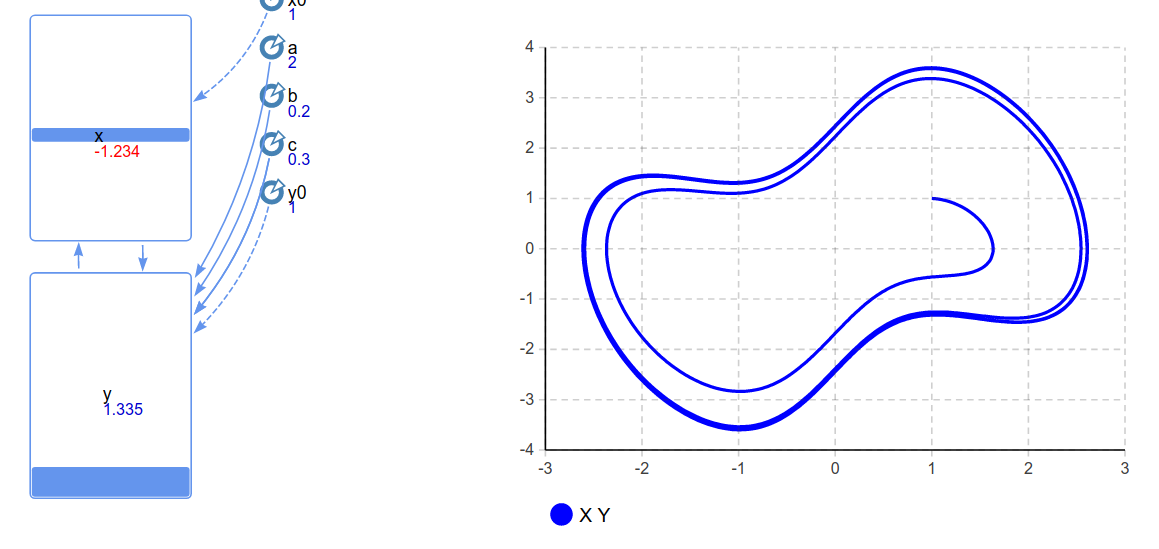
\includegraphics[scale=0.4]{goodwin1}
	\caption{Результаты построения модели Гудвина в AnyLogic: неустойчивый фокус}
	\label{fig:goodwin1}
\end{figure}

\newpage

\begin{figure}[h]
	\centering 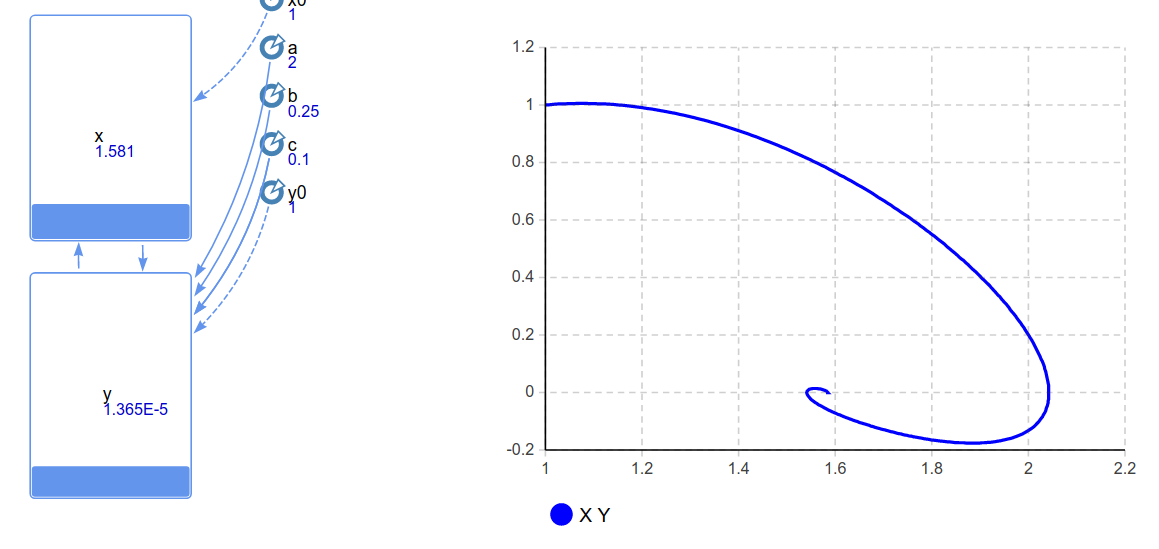
\includegraphics[scale=0.4]{goodwin2}
	\caption{Результаты построения модели Гудвина в AnyLogic: устойчивый фокус}
	\label{fig:goodwin2}
\end{figure}

Таким образом, был проведен численный и качественный анализ модели Гудвина, а так же были найдены соотношения параметров, при которых происходит бифуркация.